\section{Single user} \label{sec:single-user}

Considering a single user in the conference room, the SINR of that user will be very high compared to a scenario with more than one physically present user, as a result of experiencing no interference. Since intra-cell interference is the only interference term we may have in a single-panel single-layer transmission, the total interference is zero when a single-user is considered and the SINR degenerates in an SNR, reaching values well above the 30 dB mark.

% Section of the BLER CURVES
From the analysis of the BLER curves, previously seen in Figure \ref{fig:blercurves}, when operating with such high SINRs the probability of occurring block errors is practically zero. Hence the bit rate is either constrained by the available bits in the buffer or by the maximum possible bit rate a user can have, and we must identify which situation it is. Figure \ref{fig:su_bitrate} shows the instantaneous bit rate in each TTI and the average bit rate of the past 800 TTIs, or 200 ms, the duration of a \ac{GoP}.

\imagecapcontrol{Results/su_throughput_secs_3.5ghz.pdf}{Instantaneous and rolling average bit rate with $\overline{R}_{DL} = 80$ Mbps.}{fig:su_bitrate}{.7}{-3mm}

Note the instantaneous bit rate should resemble the packet arrival rates of Figure \ref{fig:burst}, since when there are no packets, there cannot be transmissions. The thin blue lines happen when there is no bit rate oscillations. The thick blue blocks are quick bit rate oscillations outside of the imposed by the packet arrival mechanism, e.g. right after the 0.2 and 0.4 second instants. 

We can see that these quick instantaneous bit rate oscillations happen between 145 and 190 Mbps, approximately. They occur because the buffer gets empty every TTI, and only achieve the bitrate correspondent to the number of packets available to send. Since the available packets each TTI oscillates, the bit rate does too. 

Additionally, if we perform the computation for the highest achievable bit rate under ideal conditions, i.e. no block errors on the highest \acs{MCS}, with all 50 \acsp{PRB}, we obtain that the system should support 250 Mbit/s. So, to see this number we must guarantee there are enough packets in the buffer. So, we set $\overline{R}_{DL}$ from 80 Mbps to 500 Mbps exclusively to plot the maximum achievable bit rate in Figure \ref{fig:su_bitrate_full}. 

\imagecapcontrol{Results/su_throughput_full_secs_3.5ghz.pdf}{Instantaneous and rolling average bit rate with $\overline{R}_{DL} = 500$ Mbps.}{fig:su_bitrate_full}{.73}{-3mm}

Contrary to Figure \ref{fig:su_bitrate}, there are no quick instantaneous bit rate oscillations in Figure \ref{fig:su_bitrate_full} because the number of bits in the buffer always exceeds the bits to be sent in that TTI. The zero-bit rate TTIs are due to an empty buffer - packets get discarded if the scheduler realises they are going to exceed the latency constraints and excess packets come from setting the average arrival rate so high.

Thus we may conclude that maximum average achievable bit rate for a user under the described conditions is roughly 175 Mbps, reaching 250 Mbps in instantaneous bit rate. And observe that the latency plays an important role. The higher the latency, the closer to the maximum instantaneous bit rate the average bit rate gets. 

From Figure \ref{fig:su_bitrate} we conclude the deployment and network configurations support an average bit rate of 80 Mbps in the \ac{DL} for one user. In Figure \ref{fig:su_bitrate_full} we set the threshold for what is the maximum bit rate a user can achieve. To further expand this quantity, other strategies need to be used, like using an higher MCS or multi-layer transmission.

Finally, is important to note that a conference use case with only one user is a scenario where the resource distribution is trivial and very high bit rates are expected. In the next section we consider a more demanding case of having multiple users to serve simultaneously.


\pagebreak
\section{Multiple users} \label{sec:multi-user}

Let us now consider a more demanding scenario with four physical users, each with a downlink average application bit rate of 80 Mbps. Analogously to Figure \ref{fig:su_bitrate_full}, Figure \ref{fig:mu_bitrates} represents the instantaneous bit rate as well as the average bit rate of the last 200 ms, for each present user. Here we see the a more chaotic and realistic scenario. 

\imagecapcontrol{Results/mu_throughput_secs_3.5ghz.pdf}{UE bit rates, instantaneous and averaged over the last 200 ms (GoP duration).}{fig:mu_bitrates}{.73}{-3mm}

The average quality of connections varies across users although they are placed at the same distance to the BS, uniformly distributed around the table, as described in Section \ref{sec:ue_placement}. This is due to their random head movements, and such movements change \acs{HMD} antennas' orientations, thus influencing radiations patterns, and consequently the quality of the connection and achievable bit rate.


% here the case for oscillations is block errors and channel variation
In Figure \ref{fig:mu_bitrates}, bit rate oscillations have two causes: the same as in the previous section, i.e. variability of packet arrival rate on a TTI-basis, and variability of channel conditions. In this section we carefully dissect this occurrence 

A good indicator of the channel quality variability is the SINR each user experiences. Figure \ref{fig:mu_sinr} shows the SINR estimated from channel measurements and the SINR experienced from the actual transmission. The time-varying experienced received signal power and interference power are presented in Figure \ref{fig:mu_pow}.


\imagecapcontrol{Results/mu_sinr_secs_3.5ghz.pdf}{SINR, estimated before transmission and experienced during transmission.}{fig:mu_sinr}{.73}{-3mm}

\imagecapcontrol{Results/mu_pow_vs_inter_secs_3.5ghz.pdf}{Received Signal and Interference Powers.}{fig:mu_pow}{.73}{-1mm}

\vspace{.4cm}

In Figure \ref{fig:mu_sinr} we see the estimative closely following the experienced. Note that the experienced SINR is only updated when there are transmissions, and as such it is constant for some short periods. Moreover, it agrees perfectly with Figure \ref{fig:mu_pow}. Assuming noise plays no significant role, the SINR is practically the ratio between received power and interference, and we see the SINR changing according to the signal power and interference curves. Actually, since they are in logarithmic units, the SINR is the different between the signal and interference powers.

However, Figure \ref{fig:mu_pow} also shows unexpected behaviour. It shows abnormally high received signal powers. Taking into account the \acs{BS} transmit power is 100 mW, we can see that some \acsp{UE} are receiving more than that, which is certainly wrong. However, it seems to be a problem merely with the scale because all graphs are consistent and lead to realistic \acsp{SINR}.

Nonetheless, the previous two figures are consistent. Furthermore, we see significant and unpredictable channel variations for each user. With such accentuated channel variability, the choice of MCS varies as well, which justifies variable bit rates.

Figure \ref{fig:mu_mcs} shows the \ac{MCS} index used for the transmissions to each \acs{UE}. Assuming the same degree of block errors, the higher the average MCS index, the more likely a user is to get an higher bit rate. We see this relation when comparing the achieved bit rates in Figure \ref{fig:mu_bitrates} and the MCS used for each transmission, below.

As expected, sufficient channel variability causes changes in the experienced bit rate. Furthermore, channel variability may lead to block errors, since predicting the future state of the channel is no trivial task and even the slightest drifts between SINR estimation and realisation can lead to using the incorrect MCS.

Figure \ref{fig:mu_bler} shows the running average BLER across time. And one clearly testifies that all users experience blocks with errors.

This figure agrees with what we have seen so far. For instance, in case of \ac{UE} 2, we can identify that around the 0.7 second mark the BLER monotonically decreases. This happens the SINR is so high that the highest MCS is always chosen with an estimated BLER smaller than 10\%. Indeed, by analysing the \acs{MCS} curves (Figure \ref{fig:blercurves}), we see that \acsp{SINR} above 26 dB, approximately, results in virtually no block errors, therefore driving the average BLER down. Figures \ref{fig:mu_sinr} proves that UE 2 passes this 26 dB threshold at that time.

\imagecapcontrol{Results/mu_mcs_secs_3.5ghz.pdf}{MCS index used by each UE in every transmission.}{fig:mu_mcs}{.73}{-3mm}

\imagecapcontrol{Results/running_bler_secs_3.5ghz.pdf}{All time BLER average in a multi-user scenario.}{fig:mu_bler}{.73}{-3mm}

Figure \ref{fig:mu_olla} shows the instantaneous \acs{BLER} for UE 2 and how the OLLA parameter varies accordingly. On close inspection, $\Delta_{OLLA}$ rises when there are transmissions without errors and decreases when there are transmissions where blocks had errors. This behaviour leads to choosing a lower MCS when there are errors and slowly opting for an higher MCS when the channel is better than expected. Only when there are transmissions (zones marked in grey) there are blocks with or without errors. Naturally therefore, the \acs{OLLA} parameter is not updated outside of such zones.

\begin{center}

    \hfill 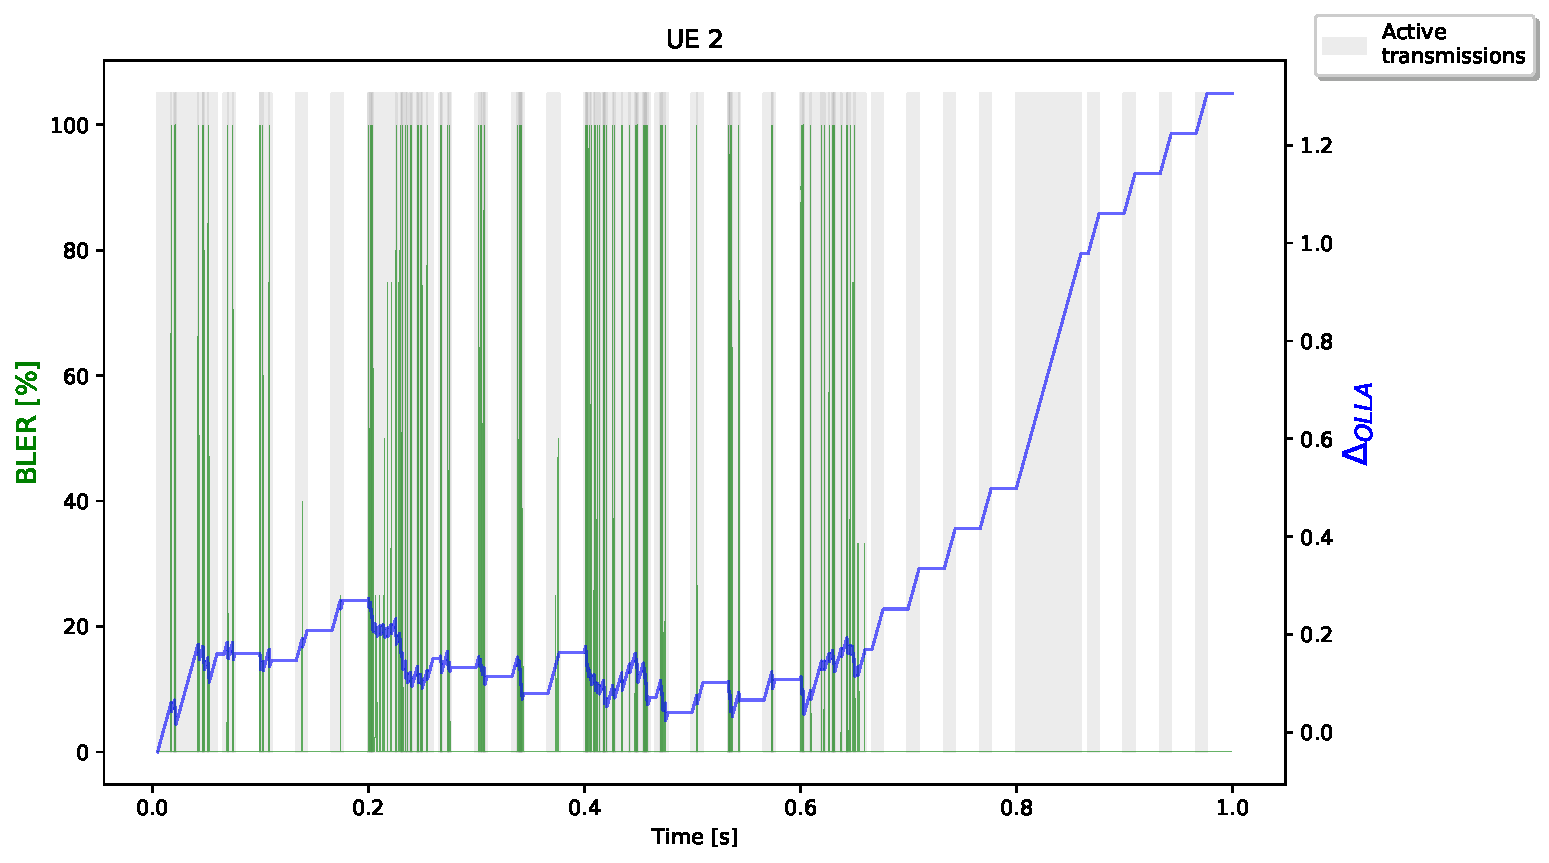
\includegraphics[scale = .59]{Results/olla_secs_3.5ghz.pdf}
    \captionsetup{type=figure} 
    \vspace{-3mm}   
    \caption{Link adaptation parameter variation with the instantaneous \acs{BLER}. Grey zones mark when the UE has active transmissions.}			
    \label{fig:mu_olla}
    
\end{center}


The use of this link adaptation scheme should make the BLER converge to the BLER target of 10\%. It still is uncertain why that does not happen. A possibility is the excessively short simulation. There are artifacts from before the convergence of the link adaptation mechanism which can drive the BLER down, and in short simulations they may still have a significant influence on the average BLER.

Finally, we can conclude regarding how well the deployment and configurations cope with the requirements. However, it should not be taken as a final statement because of the modelling simplifications listed in the beginning of this chapter, some results are yet to be understood, and this analysis lacks statistical significance: we cannot derive such conclusions by looking at one second of one use-case. But we can preliminarily conclude something about that one second despite all limiting factors.

Nevertheless, to conclude something relevant we cannot resort exclusively to bit rate plots since those say nothing about performance with respect to latencies. From the application perspective, we want to answer questions such as: ``what is maximum application throughput that achieves less than X \% packet error rate?''

A sizeable step towards answering it, and also towards improving the answer is understanding under what circumstances high packet loss occurs. 

In Figure \ref{fig:mu_lat} we see the average packet latency, i.e. average time a packet takes to be successfully sent after arriving to the buffer, and the packet drop rate on a per-frame basis. This means the horizontal axis has application frame indices - five GoP are sent per second, and each I-frame is marked in red. As a general rule, both the average packet latency and drop rate rise right after an I-frame, because those are the times where the system is under the most load. This, however, does not apply for UE2 since its channel quality is good enough to sustain the load. Nonetheless, we correlate the moment of most stress of UE 2, marked by the peak of average packet latency, with the poorest channel quality of Figure \ref{fig:mu_sinr}.

\imagecapcontrol{Results/lat_drop_rate_3.5ghz.pdf}{Packet latencies and drop-rates for all UEs with I-frame marking.}{fig:mu_lat}{.65}{-3mm}

If packets are dropped after the I frame, it means the link had enough quality to cope with the I frame, but having a P frame following with no pause led to the delay of some packets past the latency requirement. This is the case when the drop rate peak comes after the I-frame, which is the most common case. And the lower the drop rate peak is, the closer the user was to handling all packets within the required time. For instance, UE 1 has severe difficulties handling all data from the third I-frame, but is only second in performance to UE 2 in the last frame. As looking at the SINR plots in Figure \ref{fig:mu_sinr} again, we see that UE 1 has the lowest SINR at 0.4 second mark (time of third I-frame), but has the highest SINR with the exception of UE2 at the 0.8 second mark (time of the last I-frame).


